\label{recursos}
En este capítulo se tratan los recursos y las tecnologías empleadas para el
diseño y desarrollo de la aplicación Web.

\section{Angular}\label{Angular}
Angular[\url{https://angular.io}] es un framework de desarrollo web para crear
aplicaciones de una sola página (SPA) y aplicaciones web dinámicas. Fue
desarrollado por Google y se basa en el lenguaje de programación TypeScript.
\begin{figure}[htb!]
    \centering
    \caption{Logo de Angular}
    \label{fig:angular-logo}
    \centering
    
\includegraphics[scale=0.35]{./Ilustraciones/logos/Angular Logo.png}\\
    \textbf{Fuente:} Página oficial de Angular [\url{https://angular.io}]
\end{figure}
\hfill \break
Angular proporciona una estructura sólida y coherente para el desarrollo de
aplicaciones web complejas, lo que permite a los desarrolladores construir
aplicaciones de alta calidad y escalables de manera más rápida y eficiente.
Algunas de las características clave de Angular incluyen:

\textbf{Inyección de dependencias}: Permite que los componentes se comuniquen entre sí
de manera eficiente.

\textbf{Binding de datos bidireccional}: Facilita la actualización automática de la
interfaz de usuario en tiempo real.

\textbf{Directivas}: Permite crear componentes personalizados y hacer uso de componentes
predefinidos.

\textbf{Servicios}: Permite compartir datos y lógica de aplicación entre los
componentes.

Angular también viene con una amplia variedad de herramientas y bibliotecas
adicionales, como Angular CLI y Angular Material, que ayudan a los
desarrolladores a crear aplicaciones web robustas y de alta calidad.
\begin{figure}[htb!]
    \centering
    \caption{Logo de Angular Material}
    \label{fig:angularMat-logo}
    \centering
    
\includegraphics[scale=1]{./Ilustraciones/logos/Angular-Mat Logo.png}\\
    \textbf{Fuente:} Página oficial de Angular Material [\url{https://material.angular.io}]
\end{figure}
\hfill \break
Se ha hecho uso de un algunos componentes de Angular Material, como son:

Material Table
    [\url{https://v5.material.angular.io/components/table/overview}], junto con
Paginator:\\ El \textbf{componente mat-table} proporciona una tabla de datos de
estilo Material Design que se puede utilizar para mostrar filas de datos. \\ El
\textbf{componente mat-paginator} Proporciona navegación para la información
paginada, normalmente utilizada con una tabla.
\begin{figure}[htb!]
    \centering
    \caption{Muestra de tabla y paginator en Trabajo propio}
    \label{fig:tabla}
    \centering
    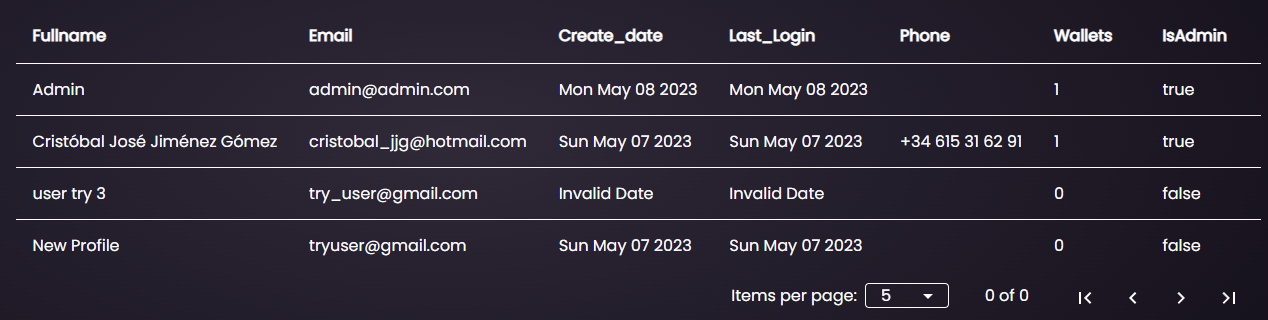
\includegraphics[scale=0.5]{./Ilustraciones/table-paginator.png}\\
    \textbf{Fuente:} Trabajo Propio en la zona de admin [\url{https://tft-galeria-nft-web3.vercel.app/admin/users}]
\end{figure}
\hfill \break

\section{Express.JS}\label{ExpressJS}
Como dicen en su propia página web, "ExpressJS es una opción rápida, sin
opiniones y minimalista para Node.js."\\ Es un popular marco de aplicación web
para Node.js que simplifica el proceso de creación de aplicaciones web y APIs
(interfaces de programación de aplicaciones). Es una capa delgada sobre Node.js
que proporciona una variedad de características y herramientas para crear
aplicaciones web y APIs de manera rápida y eficiente.
\begin{figure}[htb!]
    \centering
    \caption{Logo de ExpressJS}
    \label{fig:express-logo}
    \centering
    
\includegraphics[scale=0.5]{./Ilustraciones/logos/ExpressJS.png}\\
    \textbf{Fuente:} Página oficial de ExpressJS [\url{http://expressjs.com}]
\end{figure}
\hfill \break

ExpressJS es un marco minimalista que proporciona una estructura básica para
construir aplicaciones web, pero permite a los desarrolladores agregar
funcionalidad adicional utilizando middleware y complementos. ExpressJS también
proporciona un enrutamiento simple y flexible, lo que facilita la creación de
rutas para diferentes páginas y recursos.

Además, ExpressJS es altamente personalizable y se integra fácilmente con otros
módulos y herramientas de Node.js, lo que lo convierte en una opción popular
para construir aplicaciones web y APIs.

\section{API's}\label{APIs}
\subsection{Firebase}
\label{Firebase-desglosado}
Firebase es una plataforma de desarrollo de aplicaciones móviles y web que
ofrece una variedad de herramientas y servicios en la nube para ayudar a los
desarrolladores a crear, mejorar y escalar aplicaciones.
\begin{figure}[htb!]
    \centering
    \caption{Logo de Firebase}
    \label{fig:firebase-logo}
    \centering
    
\includegraphics[scale=0.35]{./Ilustraciones/logos/Firebase.png}\\
    \textbf{Fuente:} Página oficial de Firebase [\url{https://firebase.google.com/?hl=es}]
\end{figure}
\hfill \break
Firebase fue adquirido por Google en 2014 y desde entonces ha evolucionado para
ofrecer una amplia gama de servicios, incluyendo:
\begin{itemize}
    \item Autenticación de usuarios[Capítulo \ref{autenticacion}]: permite a los
          desarrolladores agregar fácilmente funciones de registro, inicio de sesión y
          autenticación a sus aplicaciones.
    \item Almacenamiento en la nube[Capítulo \ref{almacenamiento}]: proporciona
          almacenamiento en la nube para archivos y datos de aplicaciones.
    \item Base de datos en tiempo real: una base de datos en tiempo real en la nube que
          permite a los desarrolladores crear aplicaciones en tiempo real con
          actualizaciones automáticas y en tiempo real.
    \item Alojamiento de aplicaciones web: permite a los desarrolladores alojar sus
          aplicaciones web en los servidores de Firebase.
    \item Notificaciones push: permite enviar notificaciones push a los usuarios de la
          aplicación.
    \item Analítica de aplicaciones: proporciona análisis de usuarios y datos de uso de
          la aplicación.
\end{itemize}

Para este proyecto no se ha hecho uso de todas las utilidades, solamente de:

\subsubsection{Autenticación de usuarios}
\label{autenticacion} Se ha hecho uso de esta
utilidad debido a que nos proporciona una forma sencilla de registrar usuarios,
hacer que estos inicien sesión, y que puedan cerrar sesión de una forma simple.
Además, y como veremos en las conclusiones y trabajo futuro [Capítulo \ref{trabajo-futuro}],
nos permite hacer uso de la autenticación de Google, lo que nos permite tener
una mayor seguridad en el inicio de sesión de los usuarios.
\begin{figure}[htb!]
    \centering
    \caption{Tabla de autenticación proporcionada por Firebase}
    \label{fig:firebase-autenticacion}
    \centering
    \includegraphics[scale=0.65]{./Ilustraciones/autenticación.png}\\
    \textbf{Fuente:} Consola de Firebase, apartado de Autenticación
\end{figure}
\hfill \break

\subsubsection{Almacenamiento en la nube}
\label{almacenamiento}
Se ha hecho uso de esta utilidad debido a que nos proporciona una base de datos
en la nube, lo que nos permite tener una mayor seguridad en el almacenamiento de
los datos de los usuarios, y de la aplicación en general.
En este caso, guardamos 3 tipos de datos:
\begin{itemize}
    \item Los \textbf{usuarios} registrados, con la información del correo, si es
          administrador, el nombre, el apellido, su número de móvil, su nombre de
          usuario, que está compuesto por el inicio del correo y su primer nombre, y las
          carteras que este ha agregado.
    \item Las \textbf{colecciones} que se mostrarán de NFT's, que contienen las
          direcciones de las colecciones para poder acceder a las mismas, la url de la
          colleción, el nombre real y la foto de la marca.
    \item También se ha hecho un apartado para \textbf{mensajes}, el cual contiene
          mensajes qeu hand ejado los usuarios con intenciones de mejora. Este documento
          contiene el correo del usuario que lo ha mandado, el mensaje, y un asunto.
\end{itemize}

\begin{figure}[htb!]
    \centering
    \caption{Conjunto de colecciones y documentos proporcionada por Firebase}
    \label{fig:firebase-almacenamiento}
    \centering
    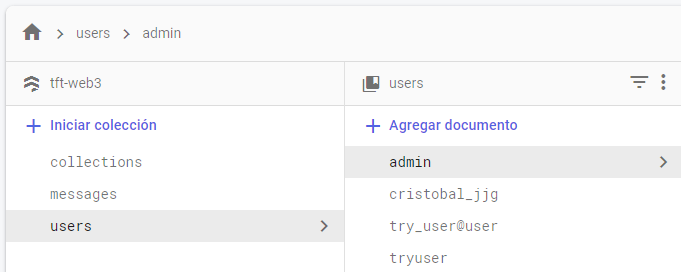
\includegraphics[scale=0.75]{./Ilustraciones/almacenamiento.png}\\
    \textbf{Fuente:} Consola de Firebase, apartado de Firestore Database
\end{figure}

\subsection{Alchemy}
\label{Alchemy-desglosado}
Alchemy es una plataforma de desarrollo con soporte multicadena y con alcance
global, pensada en facilitar el desarrollo de aplicaciones descentralizadas
(DApps). Su principal objetivo es ofrecer todo lo que los desarrolladores
necesitan para construir y hacer realidad la Web3.[\cite{alchemy}]
\begin{figure}[htb!]
    \centering
    \caption{Logo de Alchemy}
    \label{fig:alchemy-logo}
    \centering
    
\includegraphics[scale=0.5]{./Ilustraciones/logos/alchemy-logo.png}\\
    \textbf{Fuente:} Página oficial de Alchemy [\url{https://www.alchemy.com}]
\end{figure}
\hfill \break

Su relevancia en el sector le ha válido ser reconocida como el “AWS de la
Web3”, manejando más de 10 millones de usuarios, movilizando más de 100 mil
millones de dólares en activos digitales y con un concurrencia de más de 100
mil millones de requests, lo que le ha llevado a tener una valoración de
mercado de más 10 mil millones de dólares.\\

La intención de la plataforma es permitir que las aplicaciones puedan
evolucionar rápidamente para dar respuesta a las necesidades de los usuarios,
sin que esto implique la puesta en marcha de tales mejoras. Así, los
desarrolladores se pueden enfocar en lo realmente importante: diseñar y
codificar estas nuevas soluciones, confiando en que la plataforma tendrá la
flexibilidad necesaria para respaldar estos nuevos diseños y permitir que los
usuarios puedan explorarlos.

\subsection{Moralis}
\label{Moralis-desglosado}
Moralis [\url{https://moralis.io}] es una plataforma de infraestructura
blockchain de la web3 que proporciona herramientas y servicios para
desarrolladores que construyen aplicaciones descentralizadas (dApps) en la
cadena de bloques Ethereum. Ofrece una amplia gama de herramientas, incluyendo
APIs y nodos de red, para que los desarrolladores puedan interactuar con
Ethereum de manera eficiente y escalable.
\begin{figure}[htb!]
    \centering
    \caption{Logo de Moralis}
    \label{fig:moralis-logo}
    \centering
    
\includegraphics[scale=0.5]{./Ilustraciones/logos/Moralis-logo.png}\\
    \textbf{Fuente:} Página oficial de Moralis [\url{https://moralis.io}]
\end{figure}
\hfill \break

Moralis también proporciona herramientas de desarrollo para que los
desarrolladores puedan construir dApps en la cadena de bloques Ethereum de
manera más fácil y rápida. La plataforma es utilizada por una gran cantidad de
proyectos y empresas en el espacio de la web3, y es conocida por su facilidad
de uso y eficiencia en la construcción de aplicaciones descentralizadas en la
cadena de bloques Ethereum.

Entre estas empresas, podemos encontrar algunas antes nombradas, como son
Metamask[\url{https://metamask.io}] o Polygon
    [\url{https://polygon.technology}]

\section{IDE - Visual Studio Code}\label{VSCode}
Visual Studio Code (también conocido como VS Code)
[\url{https://code.visualstudio.com}] es un editor de código fuente
desarrollado por Microsoft, que es compatible con múltiples lenguajes de
programación. Está disponible de manera gratuita para Windows, Linux y macOS, y
es muy popular entre los desarrolladores por su facilidad de uso, flexibilidad
y personalización.
\begin{figure}[htb!]
      \centering
      \caption{Logo de Visual Studio Code}
      \label{fig:vscode-logo}
      \centering
      
\includegraphics[scale=0.1]{./Ilustraciones/logos/vscode-logo.png}\\
      \textbf{Fuente:} Iconduck [\url{https://iconduck.com/icons/102490/file-type-vscode}]
\end{figure}
\hfill \break

VS Code incluye características útiles como resaltado de sintaxis,
autocompletado de código, depuración de código en vivo, integración con control
de versiones y herramientas de construcción y despliegue de aplicaciones.
Además, los usuarios pueden personalizar el editor con extensiones y temas para
satisfacer sus necesidades específicas de programación.

VS Code es muy popular en el desarrollo web y en la construcción de
aplicaciones para la web3 y las criptomonedas.

Se han utilizado algunas extensiones básicas para el desarrollo web como son:
\begin{itemize}
      \item Angular Language Service [\url{https://angular.io/guide/language-service}]
      \item Auto Close Tag
                  [\url{https://marketplace.visualstudio.com/items?itemName=formulahendry.auto-close-tag}]
      \item Auto Rename Tag
                  [\url{https://marketplace.visualstudio.com/items?itemName=formulahendry.auto-rename-tag}]
      \item Console Ninja
                  [\url{https://marketplace.visualstudio.com/items?itemName=WallabyJs.console-ninja}]
      \item IntelliCode
            [\url{https://marketplace.visualstudio.com/items?itemName=VisualStudioExptTeam.vscodeintellicode}]
      \item GitHub Copilot Nightly
                  [\url{https://marketplace.visualstudio.com/items?itemName=GitHub.copilot-nightly}]
      \item Prettier - Code formatter
                  [\url{https://marketplace.visualstudio.com/items?itemName=esbenp.prettier-vscode}]
      \item SCSS Formatter
                  [\url{https://marketplace.visualstudio.com/items?itemName=sibiraj-s.vscode-scss-formatter}]
      \item VSCode-pdf
            [\url{https://marketplace.visualstudio.com/items?itemName=tomoki1207.pdf}]
\end{itemize}

\section{Trello}\label{Trello}
Trello es una herramienta de gestión de proyectos basada en la nube, que
permite a los usuarios organizar tareas y proyectos en tableros visuales y
colaborativos. Fue lanzado en 2011 y se ha vuelto muy popular entre equipos de
trabajo de diversas industrias y tamaños.
\begin{figure}[htb!]
    \centering
    \caption{Logo de Trello}
    \label{fig:trello-logo}
    \centering
    
\includegraphics[scale=0.05]{./Ilustraciones/logos/trello.1024x1024.png}\\
    \textbf{Fuente:} Iconduck [\url{https://iconduck.com/icons/95002/trello}]
\end{figure}
\hfill \break
Trello utiliza un sistema de tableros que representan los diferentes proyectos
o áreas de trabajo, y dentro de cada tablero, los usuarios pueden crear listas
de tareas y tarjetas que representan cada tarea o actividad. Estas tarjetas
pueden contener información como descripciones, listas de verificación,
etiquetas, fechas de vencimiento, comentarios y archivos adjuntos.

Además, Trello permite la colaboración entre equipos de trabajo, ya que los
miembros pueden comentar en las tarjetas, asignar tareas a otros miembros,
establecer fechas de vencimiento y recibir notificaciones de actualizaciones.
Trello también se integra con otras herramientas populares de productividad,
como Slack, Google Drive y Jira, lo que lo hace aún más útil para equipos de
trabajo que utilizan diferentes herramientas.

\section{Figma}\label{Figma}
Figma es una herramienta de diseño gráfico en línea que se utiliza para crear
interfaces de usuario, diseños de sitios web, aplicaciones móviles y otros
proyectos digitales. Fue lanzado en 2016 y se ha vuelto muy popular en la
industria del diseño debido a su capacidad para trabajar en tiempo real y
permitir la colaboración en tiempo real entre los miembros del equipo.
\begin{figure}[htb!]
    \centering
    \caption{Logo de Figma}
    \label{fig:figma-logo}
    \centering
    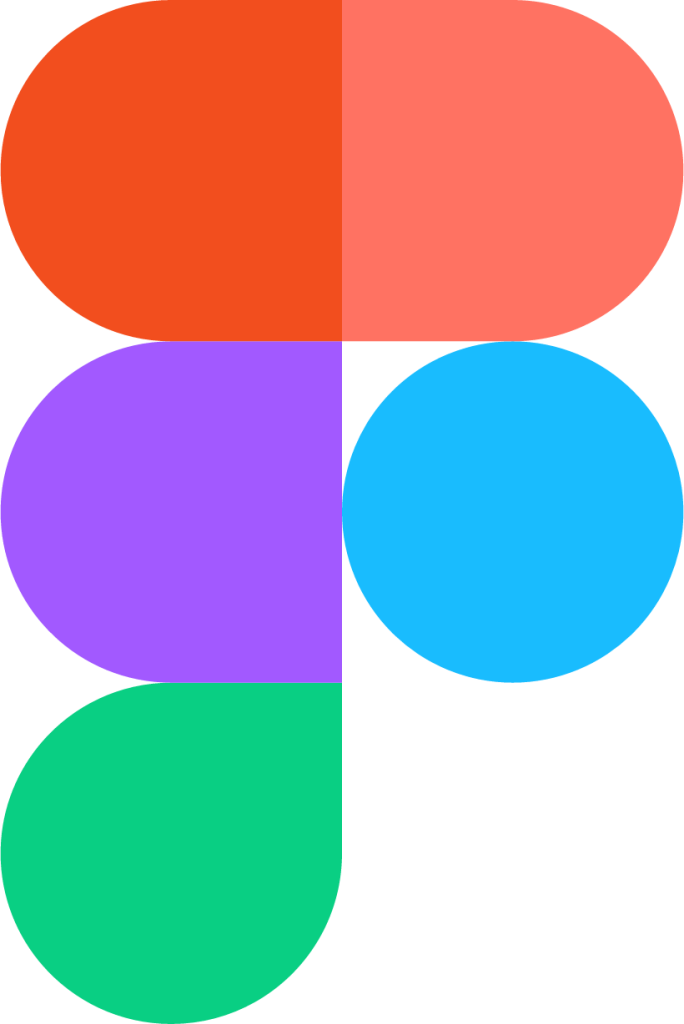
\includegraphics[scale=0.05]{./Ilustraciones/logos/figma.684x1024.png}\\
    \textbf{Fuente:} Iconduck [\url{https://iconduck.com/icons/39864/figma}]
\end{figure}
Figma nos permite crear diseños con herramientas como vectores,
formas, capas, texto y efectos, entre otras. También tiene características como
prototipado y animación, lo que lo hace ideal para diseñar interfaces interactivas.

Además, Figma es una herramienta basada en la nube, lo que significa que todos
los archivos se guardan en línea y se pueden acceder desde cualquier lugar con
conexión a Internet. Esto permite la colaboración en tiempo real entre los
miembros del equipo, ya que varios diseñadores pueden trabajar en un proyecto
simultáneamente y realizar cambios que se actualizan en tiempo real.
\section{Validaciones}\label{validaciones}
En este último curso se ha profundizado intensamente sobre la calidad del
producto y se han usado algunas herramientas para comprobar objetivamente la
calidad del mismo. En esta sección se tratarán las herramientas usadas para
validar el proyecto de forma objetiva.

\subsection{Lighthouse}\label{lighthouse}
Lighthouse es una herramienta automatizada de código abierto para mejorar el
rendimiento, la calidad y la corrección de sus aplicaciones web.

Al auditar una página, Lighthouse ejecuta un aluvión de pruebas contra la
página y luego genera un informe sobre qué tan bien lo hizo la página. Desde
aquí puede utilizar las pruebas de falla como indicadores de lo que puede hacer
para mejorar su aplicación.\cite{lighthouse-resume}

\begin{figure}[htb!]
    \centering
    \caption{Logo de Lighthouse} \label{fig:lighthouse-logo}
    \centering
    
\includegraphics[scale=0.35]{./Ilustraciones/logos/lighthouse-logo.png}\\
    \textbf{Fuente:} Chrome Web Store [\url{https://chrome.google.com/webstore/detail/lighthouse/blipmdconlkpinefehnmjammfjpmpbjk?hl=es}]
\end{figure}

Con esta herramienta se pretende obtener objetivamente una versión más
accesible de la aplicación, que los colores tengan una coherencia, sean
visibles de una forma correcta sin constrastes extraños o disonancias de tonos,
así como una ayuda a la hora de controlar el SEO de la aplicación.

\subsection{SonarQube}\label{sonarqube}
SonarQube es una herramienta de revisión de código automática y autogestionada
que ayuda sistemáticamente a entregar código limpio. SonarQube se integra en su
flujo de trabajo existente y detecta problemas en su código para ayudarlo a
realizar inspecciones continuas de código de sus proyectos. La herramienta
analiza 30+ lenguajes de programación diferentes y se integra en su
canalización de CI y plataforma DevOps para garantizar que su código cumpla con
los estándares de alta calidad\cite{sonarqube-resume}.

\begin{figure}[htb!]
    \centering
    \caption{Ciclo que propone SonarQube} \label{fig:sonar-cicle}
    \centering
    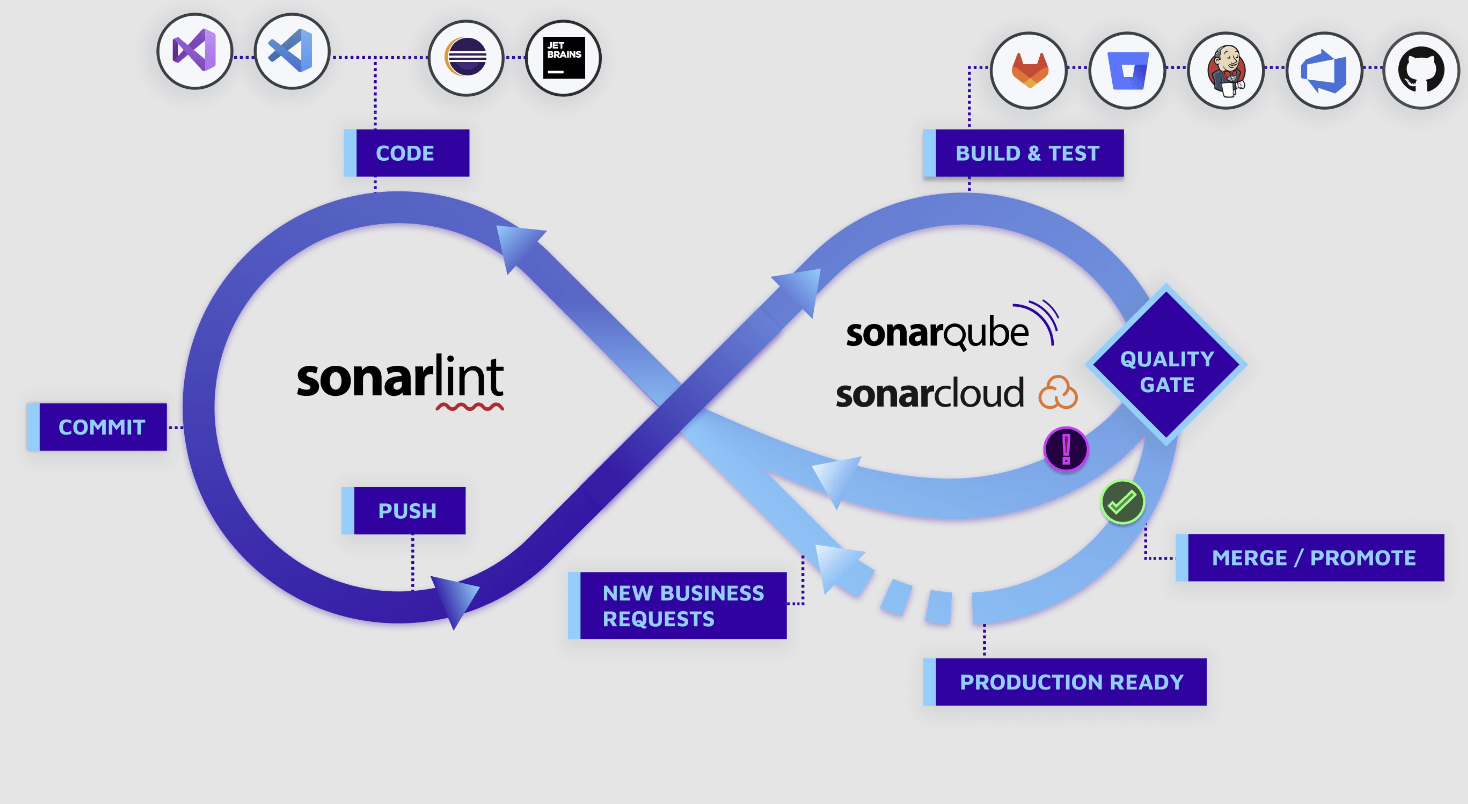
\includegraphics[scale=0.3]{./Ilustraciones/sonarqube.png}\\
    \textbf{Fuente:} Página oficial de SonarQube \url{https://docs.sonarqube.org/latest/}
\end{figure}

Con esta herramienta se pretende llegar a tener la menor cantidad de Code
Smells\footnote{El \textbf{code smell} es una indicación de la mala calidad del
código. Si hay code smells, quien lea el código tendrá la sensación de que algo
está mal. Este se soluciona refactorizando código.[\cite{code-smell}]}
posibles, así como que la deuda técnica\footnote{La \textbf{deuda técnica} es
    el costo del retrabajo adicional causado por la elección de la solución más
    rápida en lugar de la más efectiva.\cite{deuda-tecnica}} sea la menor posible.
También evitar la aparición de bugs, o vulnerabildiades en el código.
\section{Control de versiones}\label{git}
\section{Git}
La información de este apartado se ha obtenido desde la página de Atlassian
    [\url{https://www.atlassian.com/git}] \\

Git es un sistema de control de versiones gratuito y de código abierto, creado
originalmente por Linus Torvalds en 2005. Con Git, cada desarrollador tiene el
historial completo de su repositorio de código localmente. Esto hace que la
clonación inicial del repositorio sea más lenta, pero las operaciones
posteriores, como confirmar, diferenciar, fusionar y registrar, son mucho más
rápidas.
\begin{figure}[htb!]
    \centering
    \caption{Logo de Figma}\label{fig:git-logo}
    \centering
    
\includegraphics[scale=0.25]{./Ilustraciones/logos/git-logo.png}\\
    \textbf{Fuente:} Iconduck [\url{https://iconduck.com/icons/27401/git}]
\end{figure}

Git también tiene un excelente soporte para bifurcar, fusionar y reescribir el
historial del repositorio, lo que ha dado lugar a muchos flujos de trabajo y
herramientas innovadoras y potentes. Las solicitudes de incorporación de
cambios son una de esas herramientas populares que permiten a los equipos
colaborar en ramas de Git y revisar de manera eficiente el código de los demás.
Git es el sistema de control de versiones más utilizado en el mundo actual y se
considera el estándar moderno para el desarrollo de software.

Las órdenes básicas de Git son:
\begin{itemize}
    \item git init: crea un nuevo repositorio de Git vacío en el directorio actual.
    \item git clone: clona un repositorio existente en un nuevo directorio.
    \item git add: agrega cambios al área de preparación (staging area) para que estén
          listos para ser confirmados.
    \item git commit: crea un nuevo commit (instantánea) con los cambios agregados al
          área de preparación y agrega un mensaje de confirmación que describe los
          cambios.
    \item git status: muestra el estado actual del repositorio, incluyendo los cambios
          sin confirmar y los archivos sin seguimiento.
    \item git log: muestra una lista de todos los commits en orden cronológico inverso.
    \item git pull: actualiza el repositorio local con los cambios más recientes del
          repositorio remoto.
    \item git push: envía los cambios locales al repositorio remoto.
    \item git branch: muestra una lista de todas las ramas en el repositorio.
    \item git checkout: cambia a otra rama o commit.
\end{itemize}

\section{GitKraken}\label{git-kraken}
GitKraken es una herramienta de gestión de versiones de código que ofrece una
interfaz visual y fácil de usar para trabajar con Git. Es una aplicación de
escritorio que permite a los desarrolladores y equipos de desarrollo colaborar
en proyectos de software de manera eficiente.

Con GitKraken, se pueden realizar operaciones comunes de Git, como hacer
commits, fusionar ramas, crear y clonar repositorios, y gestionar conflictos de
fusión.

Además, cuenta con características adicionales, como la posibilidad de
integrarse con plataformas de gestión de proyectos como Trello, la capacidad de
ver el historial de cambios en el código, y la opción de visualizar y comparar
ramas de Git.

Grandes empresas hacen uso de esta herramienta, empesas tales como Netflix,
Philips, Amazon, Unity y Disney entre otras.

\begin{figure}[htb!]
    \centering
    \caption{Logo de Figma}\label{fig:gitkraken-logo}
    \centering
    
\includegraphics[scale=0.15]{./Ilustraciones/logos/gitkraken-logo.png}\\
    \textbf{Fuente:} Iconduck [\url{https://iconduck.com/icons/27407/gitkraken}]
\end{figure}